\documentclass[tikz,border=1pt]{standalone}
\usepackage[T1]{fontenc}
\usepackage{amsmath}
\usepackage{newtxtext,newtxmath}
\usepackage{pifont}
\usetikzlibrary{arrows.meta,positioning,calc,fit,backgrounds,patterns,patterns.meta,shapes.geometric,shapes.misc}

% Okabe-Ito colourblind-safe palette (one colour per method in every figure)
\definecolor{oiBlue}{HTML}{0072B2}
\definecolor{oiVermilion}{HTML}{D55E00}
\definecolor{oiGreen}{HTML}{009E73}
\definecolor{oiOrange}{HTML}{E69F00}
\definecolor{oiPurple}{HTML}{CC79A7}
\definecolor{oiSky}{HTML}{56B4E9}
\definecolor{oiYellow}{HTML}{F0E442}
\definecolor{oiGrey}{HTML}{8C8C8C}
\definecolor{oiGrid}{HTML}{D9D9D9}
\definecolor{oiInk}{HTML}{1A1A1A}

\newcommand{\okmark}{\textcolor{oiGreen!70!black}{\ding{51}}}
\newcommand{\badmark}{\textcolor{oiVermilion}{\ding{55}}}
\newcommand{\cellfont}{\fontsize{6.5}{7.6}\selectfont}

\tikzset{
  >={Latex[length=1.7mm,width=1.4mm]},
  flow/.style={->, line width=0.6pt, draw=oiInk},
  hatch/.style={pattern={Lines[angle=45,distance=2.4pt,line width=0.35pt]}, pattern color=black!28},
}

\tikzset{subcap/.style={font=\footnotesize, anchor=north, inner sep=0pt}}
\begin{document}
\renewcommand{\cellfont}{\fontsize{8.5}{9.7}\selectfont}
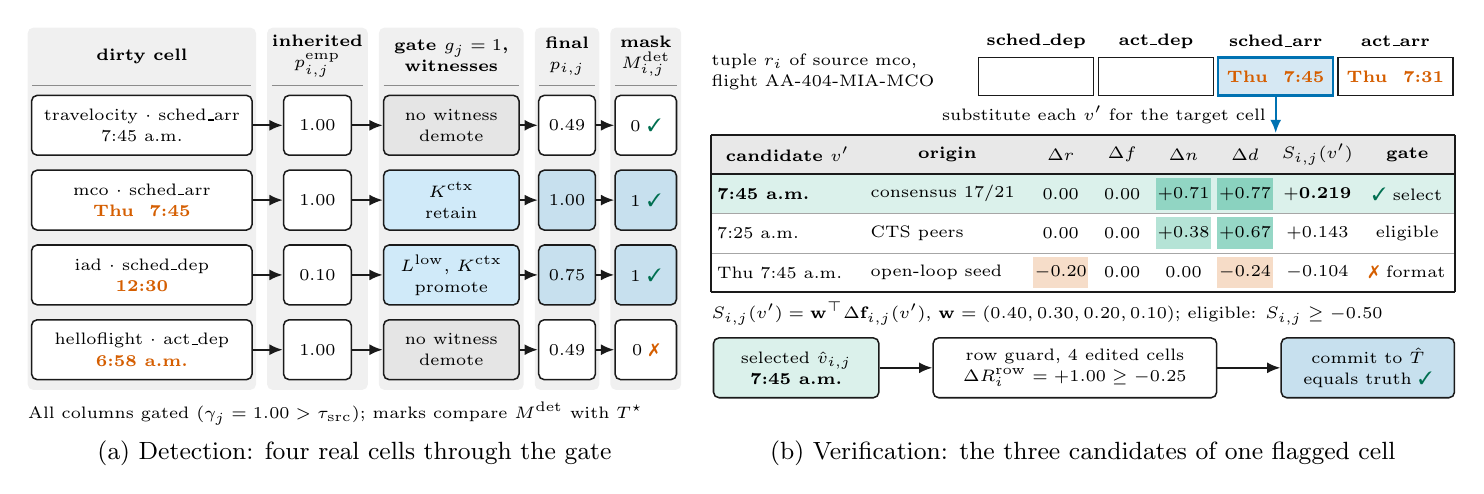
\begin{tikzpicture}[x=1cm,y=1cm, font=\cellfont,
  flow/.style={->, line width=0.8pt, draw=oiInk},
  subcap/.style={font=\fontsize{9}{10.6}\selectfont, anchor=north, inner sep=0pt},
  chip/.style={draw=oiInk, line width=0.55pt, rounded corners=2pt, inner sep=1.6pt, align=center, fill=white, minimum height=0.76cm},
  head/.style={font=\cellfont\bfseries, inner sep=0pt, align=center}]
\fill[black!6, rounded corners=2pt] (0.00,0.70) rectangle (2.90,5.30);
\node[head] at (1.45,4.94) {dirty cell};
\draw[line width=0.4pt, draw=black!45] (0.06,4.57) -- (2.84,4.57);
\fill[black!6, rounded corners=2pt] (3.04,0.70) rectangle (4.32,5.30);
\node[head] at (3.68,4.94) {inherited\\$p^{\mathrm{emp}}_{i,j}$};
\draw[line width=0.4pt, draw=black!45] (3.10,4.57) -- (4.26,4.57);
\fill[black!6, rounded corners=2pt] (4.46,0.70) rectangle (6.30,5.30);
\node[head] at (5.38,4.94) {gate $g_j = 1$,\\witnesses};
\draw[line width=0.4pt, draw=black!45] (4.52,4.57) -- (6.24,4.57);
\fill[black!6, rounded corners=2pt] (6.44,0.70) rectangle (7.26,5.30);
\node[head] at (6.85,4.94) {final\\$p_{i,j}$};
\draw[line width=0.4pt, draw=black!45] (6.50,4.57) -- (7.20,4.57);
\fill[black!6, rounded corners=2pt] (7.40,0.70) rectangle (8.30,5.30);
\node[head] at (7.85,4.94) {mask\\$M^{\mathrm{det}}_{i,j}$};
\draw[line width=0.4pt, draw=black!45] (7.46,4.57) -- (8.24,4.57);
\node[chip, minimum width=2.80cm] (c) at (1.450,4.06) {travelocity $\cdot$ sched\_arr\\{7:45 a.m.}};
\node[chip, minimum width=0.86cm] (i) at (3.680,4.06) {1.00};
\node[chip, minimum width=1.72cm, fill=black!10] (w) at (5.380,4.06) {no witness\\demote};
\node[chip, minimum width=0.72cm, fill=white] (f) at (6.850,4.06) {0.49};
\node[chip, minimum width=0.78cm, fill=white] (m) at (7.850,4.06) {0~\okmark};
\draw[flow] (c) -- (i); \draw[flow] (i) -- (w); \draw[flow] (w) -- (f); \draw[flow] (f) -- (m);
\node[chip, minimum width=2.80cm] (c) at (1.450,3.11) {mco $\cdot$ sched\_arr\\{\bfseries\color{oiVermilion}Thu ~7:45}};
\node[chip, minimum width=0.86cm] (i) at (3.680,3.11) {1.00};
\node[chip, minimum width=1.72cm, fill=oiSky!28] (w) at (5.380,3.11) {$K^{\mathrm{ctx}}$\\retain};
\node[chip, minimum width=0.72cm, fill=oiBlue!22] (f) at (6.850,3.11) {1.00};
\node[chip, minimum width=0.78cm, fill=oiBlue!22] (m) at (7.850,3.11) {1~\okmark};
\draw[flow] (c) -- (i); \draw[flow] (i) -- (w); \draw[flow] (w) -- (f); \draw[flow] (f) -- (m);
\node[chip, minimum width=2.80cm] (c) at (1.450,2.16) {iad $\cdot$ sched\_dep\\{\bfseries\color{oiVermilion}12:30}};
\node[chip, minimum width=0.86cm] (i) at (3.680,2.16) {0.10};
\node[chip, minimum width=1.72cm, fill=oiSky!28] (w) at (5.380,2.16) {$L^{\mathrm{low}}$, $K^{\mathrm{ctx}}$\\promote};
\node[chip, minimum width=0.72cm, fill=oiBlue!22] (f) at (6.850,2.16) {0.75};
\node[chip, minimum width=0.78cm, fill=oiBlue!22] (m) at (7.850,2.16) {1~\okmark};
\draw[flow] (c) -- (i); \draw[flow] (i) -- (w); \draw[flow] (w) -- (f); \draw[flow] (f) -- (m);
\node[chip, minimum width=2.80cm] (c) at (1.450,1.21) {helloflight $\cdot$ act\_dep\\{\bfseries\color{oiVermilion}6:58 a.m.}};
\node[chip, minimum width=0.86cm] (i) at (3.680,1.21) {1.00};
\node[chip, minimum width=1.72cm, fill=black!10] (w) at (5.380,1.21) {no witness\\demote};
\node[chip, minimum width=0.72cm, fill=white] (f) at (6.850,1.21) {0.49};
\node[chip, minimum width=0.78cm, fill=white] (m) at (7.850,1.21) {0~\badmark};
\draw[flow] (c) -- (i); \draw[flow] (i) -- (w); \draw[flow] (w) -- (f); \draw[flow] (f) -- (m);
\node[anchor=west, inner sep=0pt] at (0,0.40) {All columns gated ($\gamma_j = 1.00 > \tau_{\mathrm{src}}$); marks compare $M^{\mathrm{det}}$ with $T^{\star}$};
\node[subcap] at (4.15,0.06) {(a) Detection: four real cells through the gate};
\begin{scope}[shift={(8.68,0)}]
\node[anchor=west, inner sep=0pt, align=left] at (0,4.74) {tuple $r_i$ of source mco,\\flight AA-404-MIA-MCO};
\node[inner sep=0pt, font=\cellfont\bfseries] at (4.13,5.13) {sched\_dep};
\draw[line width=0.45pt, draw=oiInk, fill=white] (3.40,4.44) rectangle (4.86,4.92);
\node[inner sep=0pt] at (4.13,4.68) {\bfseries\color{oiVermilion}$\varnothing$};
\node[inner sep=0pt, font=\cellfont\bfseries] at (5.65,5.13) {act\_dep};
\draw[line width=0.45pt, draw=oiInk, fill=white] (4.92,4.44) rectangle (6.38,4.92);
\node[inner sep=0pt] at (5.65,4.68) {\bfseries\color{oiVermilion}$\varnothing$};
\node[inner sep=0pt, font=\cellfont\bfseries] at (7.17,5.13) {sched\_arr};
\draw[line width=0.9pt, draw=oiBlue, fill=oiBlue!16] (6.44,4.44) rectangle (7.90,4.92);
\node[inner sep=0pt] at (7.17,4.68) {\bfseries\color{oiVermilion}Thu ~7:45};
\node[inner sep=0pt, font=\cellfont\bfseries] at (8.69,5.13) {act\_arr};
\draw[line width=0.45pt, draw=oiInk, fill=white] (7.96,4.44) rectangle (9.42,4.92);
\node[inner sep=0pt] at (8.69,4.68) {\bfseries\color{oiVermilion}Thu ~7:31};
\fill[black!9] (0,3.44) rectangle (9.45,3.94);
\node[head] at (0.97,3.69) {candidate $v'$};
\node[head] at (3.00,3.69) {origin};
\node[head] at (4.44,3.69) {$\Delta r$};
\node[head] at (5.22,3.69) {$\Delta f$};
\node[head] at (6.00,3.69) {$\Delta n$};
\node[head] at (6.78,3.69) {$\Delta d$};
\node[head] at (7.70,3.69) {$S_{i,j}(v')$};
\node[head] at (8.84,3.69) {gate};
\draw[flow, draw=oiBlue] (7.17,4.44) -- (7.17,3.96);
\node[anchor=east, inner sep=0pt] at (7.05,4.19) {substitute each $v'$ for the target cell};
\fill[oiGreen!14] (0,2.94) rectangle (9.45,3.44);
\node[anchor=west, inner sep=0pt] at (0.07,3.19) {\bfseries 7:45 a.m.};
\node[anchor=west, inner sep=0pt] at (2.02,3.19) {consensus 17/21};
\node[inner sep=0pt] at (4.44,3.19) {0.00};
\node[inner sep=0pt] at (5.22,3.19) {0.00};
\fill[oiGreen!43] (5.65,2.99) rectangle (6.35,3.39);
\node[inner sep=0pt] at (6.00,3.19) {$+$0.71};
\fill[oiGreen!46] (6.43,2.99) rectangle (7.13,3.39);
\node[inner sep=0pt] at (6.78,3.19) {$+$0.77};
\node[inner sep=0pt] at (7.70,3.19) {\bfseries $+$0.219};
\node[inner sep=0pt] at (8.84,3.19) {\okmark~select};
\node[anchor=west, inner sep=0pt] at (0.07,2.69) {7:25 a.m.};
\node[anchor=west, inner sep=0pt] at (2.02,2.69) {CTS peers};
\node[inner sep=0pt] at (4.44,2.69) {0.00};
\node[inner sep=0pt] at (5.22,2.69) {0.00};
\fill[oiGreen!29] (5.65,2.49) rectangle (6.35,2.89);
\node[inner sep=0pt] at (6.00,2.69) {$+$0.38};
\fill[oiGreen!41] (6.43,2.49) rectangle (7.13,2.89);
\node[inner sep=0pt] at (6.78,2.69) {$+$0.67};
\node[inner sep=0pt] at (7.70,2.69) {$+$0.143};
\node[inner sep=0pt] at (8.84,2.69) {eligible};
\node[anchor=west, inner sep=0pt] at (0.07,2.19) {Thu 7:45 a.m.};
\node[anchor=west, inner sep=0pt] at (2.02,2.19) {open-loop seed};
\fill[oiVermilion!21] (4.09,1.99) rectangle (4.79,2.39);
\node[inner sep=0pt] at (4.44,2.19) {$-$0.20};
\node[inner sep=0pt] at (5.22,2.19) {0.00};
\node[inner sep=0pt] at (6.00,2.19) {0.00};
\fill[oiVermilion!22] (6.43,1.99) rectangle (7.13,2.39);
\node[inner sep=0pt] at (6.78,2.19) {$-$0.24};
\node[inner sep=0pt] at (7.70,2.19) {$-$0.104};
\node[inner sep=0pt] at (8.84,2.19) {\badmark~format};
\draw[line width=0.6pt, draw=oiInk] (0,3.94) -- (9.45,3.94);
\draw[line width=0.6pt, draw=oiInk] (0,3.44) -- (9.45,3.44);
\draw[line width=0.25pt, draw=black!35] (0,2.94) -- (9.45,2.94);
\draw[line width=0.25pt, draw=black!35] (0,2.44) -- (9.45,2.44);
\draw[line width=0.6pt, draw=oiInk] (0,1.94) -- (9.45,1.94);
\draw[line width=0.6pt, draw=oiInk] (0,3.94) -- (0,1.94) (9.45,3.94) -- (9.45,1.94);
\node[anchor=west, inner sep=0pt] at (0,1.67) {$S_{i,j}(v') = \mathbf{w}^{\top}\Delta\mathbf{f}_{i,j}(v')$, $\mathbf{w} = (0.40, 0.30, 0.20, 0.10)$; eligible: $S_{i,j} \ge -0.50$};
\node[chip, minimum width=2.10cm, fill=oiGreen!14] (s) at (1.08,0.98) {selected $\hat{v}_{i,j}$\\{\bfseries 7:45 a.m.}};
\node[chip, minimum width=3.60cm] (g) at (4.62,0.98) {row guard, 4 edited cells\\$\Delta R_i^{\mathrm{row}} = +1.00 \ge -0.25$};
\node[chip, minimum width=2.20cm, fill=oiBlue!22] (k) at (8.34,0.98) {commit to $\hat{T}$\\equals truth \okmark};
\draw[flow] (s) -- (g); \draw[flow] (g) -- (k);
\node[subcap] at (4.72,0.06) {(b) Verification: the three candidates of one flagged cell};
\end{scope}
\end{tikzpicture}
\end{document}
